\documentclass[10pt,a4paper]{article}

%double si on veut une version prof et une version élève. simple si on veut une seule version.
\newcommand{\buildmode}{double}

\InputIfFileExists{version.tex}{}{}
% Version (définie par le script)
\providecommand{\version}{eleve}

\usepackage{feuilleactivite}

%%%à modifier à chaque fois

\renewcommand{\niveau}{2nde}
\renewcommand{\chapitre}{Fonctions affines}
\renewcommand{\numchap}{0.4} 
\renewcommand{\theme}{Fonctions}

\begin{document}

\begin{objectifs}
\begin{itemize}
    \item Réactiver les notions de fonctions affines.
    \item Comprendre l'influence du coefficent directeur et de l'ordonnée à l'origine. 
    \item Représenter graphiquement une fonction affine.
\end{itemize}
\end{objectifs}

\prof{
    Au préalable, rappeler ce qu'est une fonction affine : formule \(f(x) = ax+b\) puis vocabulaire \(a\) et \(b\).\\
    Après l'activité, enchainer sur le cours : définition d'une fonction affine, coef directeur et ordonnée à l'origine.
}

\begin{exo}
\begin{enumerate}
    \item
\begin{multicols}{2}
Soient $f$, $g$ et $h$ trois fonctions définies sur $\R$ telles que $f(x)=2x$, $g(x)=-2x+3$, $h(x)=5$.

Remplir les fonctions ci-dessous et représenter ces fonctions dans le repère ci-contre :

 \setlength{\tabcolsep}{10pt}
\renewcommand{\arraystretch}{1.5}
\begin{tabular}{|c|c|c|c|c|c|c|c|}
\hline
$x$ & -3 & -2 & -1 & 0 & 1 & 2 & 3 \\
\hline
$f(x)$&  &    &    &   &   &   &   \\
\hline
\end{tabular}

\begin{tabular}{|c|c|c|c|c|c|c|c|}
\hline
$x$ & -3 & -2 & -1 & 0 & 1 & 2 & 3 \\
\hline
$g(x)$&  &    &    &   &   &   &   \\
\hline
\end{tabular}

\begin{tabular}{|c|c|c|c|c|c|c|c|}
\hline
$x$ & -3 & -2 & -1 & 0 & 1 & 2 & 3 \\
\hline
$h(x)$&  &    &    &   &   &   &   \\
\hline
\end{tabular}

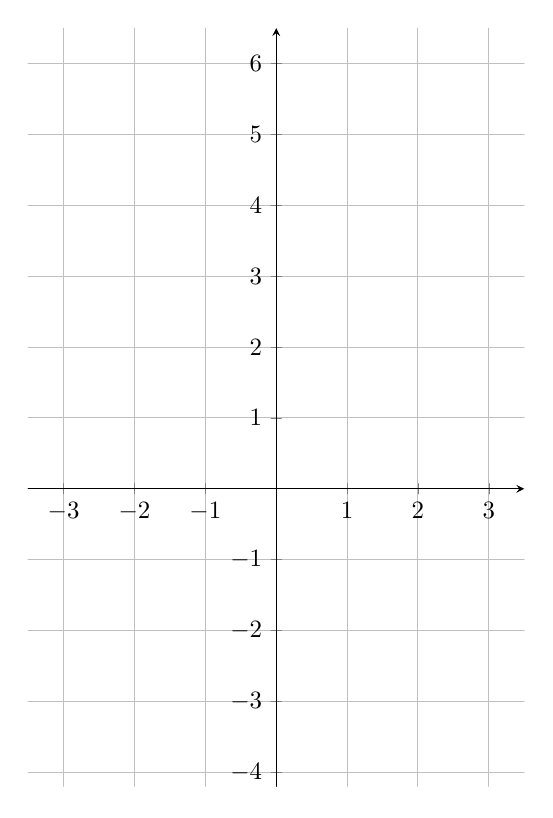
\begin{tikzpicture}[line cap=round,line join=round 45,x=1cm,y=1cm, scale=0.9]
\begin{axis}[
x=1cm,y=1cm,
axis lines=middle,
ymajorgrids=true,
xmajorgrids=true,
xmin=-3.5,
xmax=3.5,
ymin=-4.2,
ymax=6.5,
xtick={-7,-6,...,8},
ytick={-4,-3,...,8},]
\clip(-7.924912946558353,-4.660030276269421) rectangle (8.604968540093015,5.645775780210352);
\draw (-7.789606958945927,4.050292676280496) node {$f$};
\end{axis}
\end{tikzpicture} 
\end{multicols}

\item Sur le graphique ci-dessus, représenter, avec des couleurs différentes, le coefficient directeur et l'ordonnée à l'origine de chaque droite.

\item Parmi les tableaux ci-dessus, le(s)quel(s) sont des tableaux de proportionnalité ?
 \end{enumerate}
\end{exo}

\begin{multicols}{2}
\begin{exo}[][]
\(f\) est une fonction qui s'écrit \(f(x) = ax+b\) (donc c'est une fonction affine).
\begin{enumerate}
    \item Rappeler la définition du signe d'un nombre.
    \item Relier les points correspondants dans le tableau ci-contre.
    
    \renewcommand{\arraystretch}{3}
    \begin{tabular}{|rcp{1cm}cp{2.5cm}|}
        \hline
        \(f(x)=ax+b\) &  & & & Représentation graphique de \(f\) \\[0.3cm] \hline
        \(a<0\) et \(b<0\) & \(\bullet\) &  & \(\bullet\) &         \vspace{-0.7cm}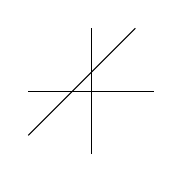
\begin{tikzpicture}[scale=0.8]
            \draw(-1,0)--(1,0);
            \draw(0,-1)--(0,1);
            \draw (-1,-0.7)--(0.7,1);
        \end{tikzpicture} \\
        \(a<0\) et \(b>0\) & \(\bullet\) &  & \(\bullet\) &         \vspace{-1cm}\begin{tikzpicture}[scale=0.8]
            \draw(-1,0)--(1,0);
            \draw(0,-1)--(0,1);
            \draw (-1,0.7)--(0.7,-1);
        \end{tikzpicture} \\
        \(a>0\) et \(b<0\) & \(\bullet\) &  & \(\bullet\) &         \vspace{-1cm}\begin{tikzpicture}[scale=0.8]
            \draw(-1,0)--(1,0);
            \draw(0,-1)--(0,1);
            \draw (-0.7,1)--(1,-0.7);
        \end{tikzpicture} \\
        \(a<0\) et \(b<0\) & \(\bullet\) &  & \(\bullet\) &         \vspace{-1cm}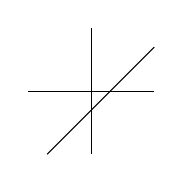
\begin{tikzpicture}[scale=0.8]
            \draw(-1,0)--(1,0);
            \draw(0,-1)--(0,1);
            \draw (-0.7,-1)--(1,0.7);
        \end{tikzpicture} \\
        \hline
    \end{tabular}
\end{enumerate}
\end{exo}
\end{multicols}

%\legendeicones

\vspace{-0.3cm}


\end{document}
